\section{Challenges in Creating Data Comics}
\label{sec:data_comics}
\begin{figure}
 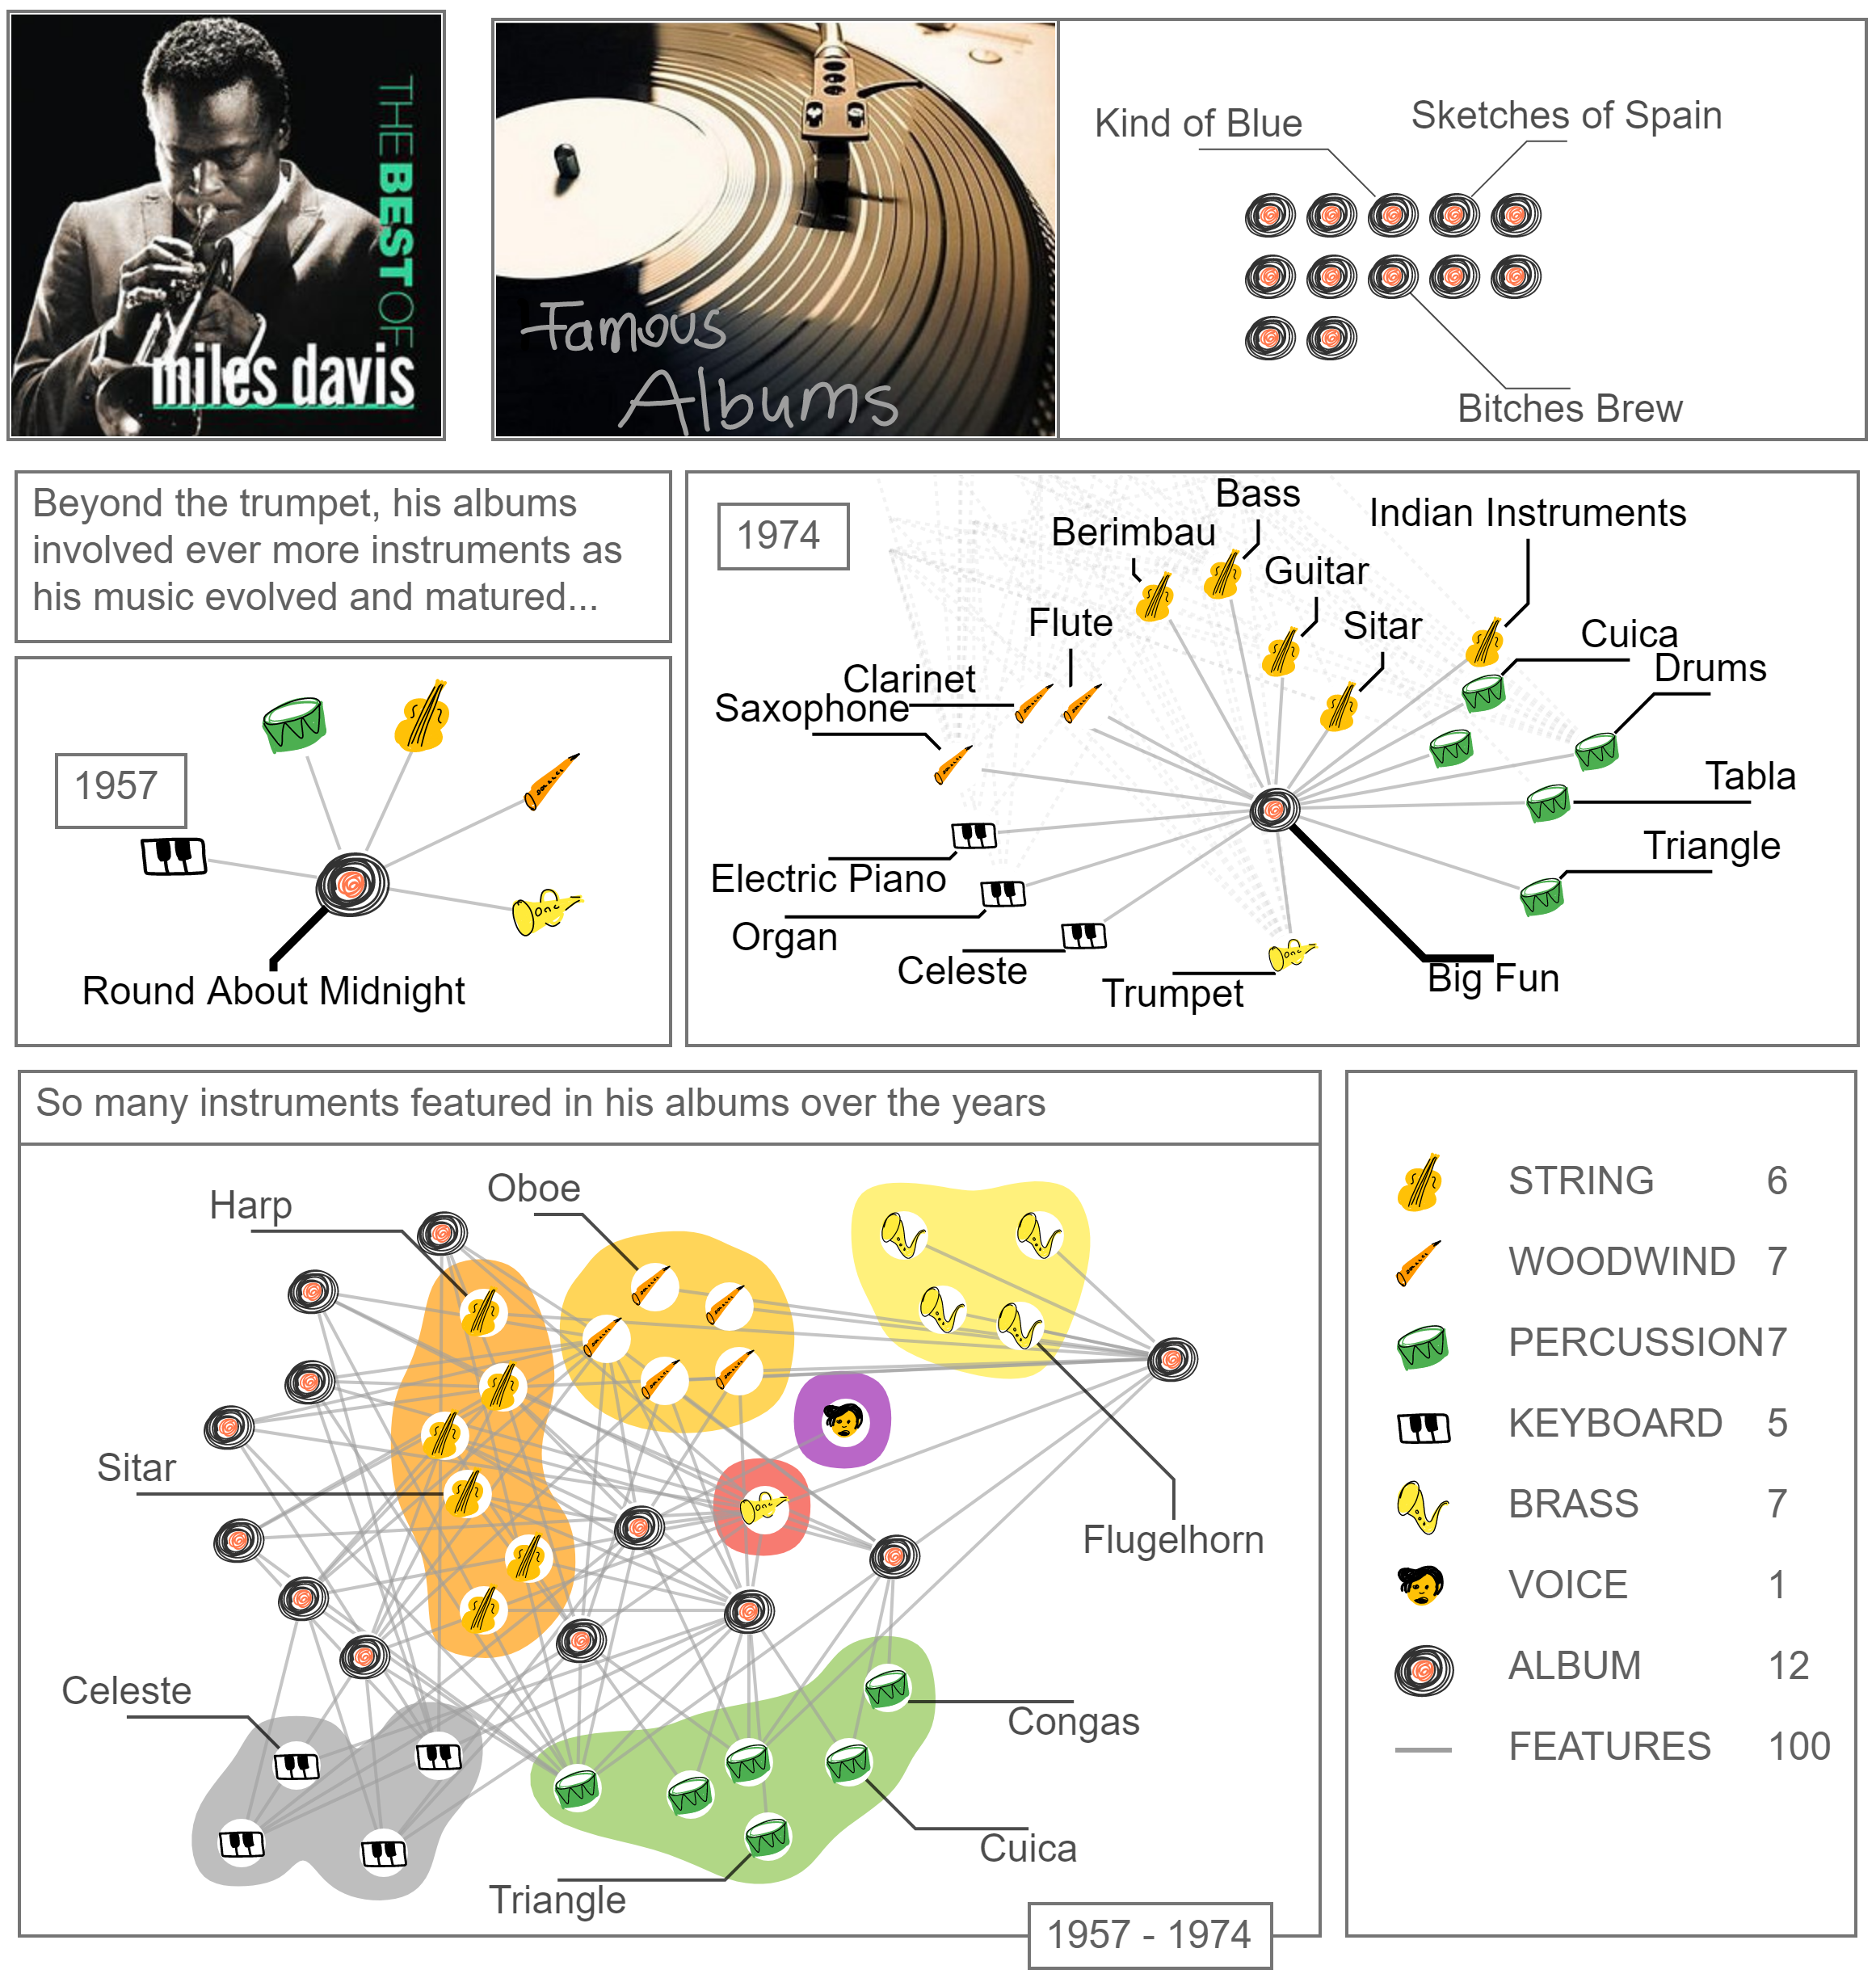
\includegraphics[width=\columnwidth]{figures/datacomic.png}
  \caption{Data Comics created with our tool and used a study material. \nat{we can potentially label elements and refer to them in 2}}
\end{figure}

To streamline our research and the design of \toolname, we first revisit the main components of comics and reflect on the challenges in creating data comics, based on common sense and our own experience in creating and researching data comics. We then look into their current (unsatisfying) support through existing authoring environments for comics and data-driven storytelling, none of which explicitly designed for data comics.

Comics is a well-established storytelling medium and has been widely applied in a variety of domains due to its versatility and familiarity. Comics have been used in storyboarding~\cite{haesen2010draw,moraveji2007comicboarding}, science education~\cite{green2010graphic,tatalovic2009science}, and information communication~\cite{caldwell2012information}. McCloud, a comics theorist, describe comics as \textit{juxtaposed pictorial and other images in deliberate sequence, intended to convey information to the viewer}~\cite{mccloud1993understanding} or, to put it simply, \textit{sequential art}~\cite{mccloud1993understanding,eisner2008comics}. It is distinct from animation or video in that images in such form are sequential in time not spatially juxtaposed as comics are~\cite{mccloud1993understanding,groensteen2007system}.

Data comics employ visualizations to communicate about data and narration to explain visualizations, context, and insights. From this synergy of data, data visualization, comics, and narration, we can describe the following challenges for computer-aided authoring support.

\textbf{C1: Integrating Words and Visualizations}---Words and pictures together make the vocabulary of comics~\cite{mccloud1993understanding}. The way in which words and pictures cooperate is unique in comics (e.g., word-specific, picture-specific, and inter-dependent combinations)~\cite{saraceni2003language,mccloud1993understanding}. Words in comics are mostly represented as \textit{speech balloons} or \textit{captions}, while often integrated into pictures and treated graphically to convey moods or sounds (e.g, onomatopoeia) ~\cite{eisner2008comics}. Pictures can take different levels of representations from realistic to abstract. 

\ben{To related work?:}
In data comics, visualization and annotation are special forms of words and pictures. The current dichotomy between visualization construction tools and graphic design tools prevent effectively balancing these two, which is critical to data comics. This is akin to the authoring of infographics. Existing visualization tools lack support for generating custom styles and adding freeform graphical elements, forcing designers to go back and forth with graphic design tools~\cite{bigelow2017iterating}.


% (e.g., information visualization is iconic and abstract). 

% \nat{This is akin to infographics. This is why data visualization tools are not enough, they do not help generate the style (e.g. drawing, import shape per data points) and the words (labels, titles captions, etc). So designers have to go back and forth with graphic tools like illustrator~\cite{bigelow2017iterating}.}

\textbf{C2: Managing multiple panels}---A panel is a basic communication unit for comics, serving as an window of information. Panels are mostly represented as framed rectangles and arranged in an orderly fashion. Each panel represents a delimited space and time in the narrative and controls the duration of attention and affects the pacing of the narration~\cite{caldwell2012comic,duncan2000toward,duncan2015power}. It may have a different size, shape, border style (e.g., inset or vignette), which can induce a different reading experience. For example, a long stretched panel creates a feeling of a long time span~\cite{eisner2008comics}).

Managing and arranging multiple panels of visualizations is important in data comics but not addressed well in existing tools. For example, a user may want to break down the complexity of data into multiples to focus on one aspect of the data at a time and progressively reveal the narrative. This story authoring aspect requires more thoughtful design than merely supporting the creation of multiple visualizations. Bach et al. identified different design patterns of panel layouts and content relations between panels to further explore the dimensions of flow and narration~\cite{bachdesign}. These patterns suggest the expressive potential of data comics to meet different narrative styles and structures. 

% \nat{For data comics, the challenge is to accurately represent the underlying data. You have to do it many times. Also you cannot show the exact same data in each panel or it would be busy, so you need to break it down, show some progression. Example of element identify, figure 8 in our graph comics paper, also vary level of details depending on what the insight is Figure 9 graph comics paper}


\textbf{C3: Create understandable transitions}
The panels are spatially juxtaposed to convey both time and space (i.e., temporal mapping), offering a jagged, staccato rhythm of unconnected moments~\cite{mccloud1993understanding}. The white space separating two consecutive panels is called the \textit{gutter} in which readers use their imagination to fill the gap between the isolated moments~\cite{mccloud1993understanding}. This process of reading is called \textit{closure}, the phenomenon of observing the parts but perceiving the whole~\cite{mccloud1993understanding,duncan2015power}.

Creating transitions to progress the narrative often requires a lot of duplication of panels and minor modifications in between the panels, as a data comic author frequently has to decide what moments to encapsulate into the panels. For example, starting from an overview panel, the author may want to focus on a detail in the next panel. To guide the reader, the author has to create transitions and control how fast or slow zooming is, which requires many trials of creating panels with different zoom factors. 


% \nat{Creating transitions introduces a lot of duplication to help people fill the gap between comics. with minor modifications in between.}
%\paragraph{Transitions}
%The composition and arrangement of panels create the \textit{grammar of comics}~\cite{eisner2008comics}. McCloud discusses six transitions that are common in traditional comics: \textit{moment-to-moment, action-to-ction, subject-to-subject, aspect-to-aspect, and non-sequitur}. Others suggested a different taxonomy based on spatio-temporality~\cite{cohn2003syntatic}. If panels in transitions are far apart in time or space, it would require more cognitive efforts to generate closure; in such cases, captions or dialogues can be used to aid understanding.


% \textbf{C4: Layout and size panels}
% The transitions between adjacent panels does not take into account the global layout of the panels on a page~\cite{caldwell2012comic}. The layout does not change the meaning but perception of the narrative (e.g., pacing, reading order)~\cite{cohn2014architecture}. For instance, when two vertically stacked panels are directly adjacent to a long vertical panel spanning the previous two, blockage can occur and confuse readers to deviate from a conventional reading order~\cite{cohn2014architecture}. A canonical grid is most popularly used~\cite{postema2013narrative,abel2008drawing} while other variations are possible such as staggered and overlapping panels~\cite{cohn2014architecture}. 
% Bach et al. identified different design patterns of panel layouts and content relations between panels to further explore the dimensions of flow and narration~\cite{bachdesign}. These patterns suggest the expressive potential of data comics to meet different narrative styles and structures. 


Finding the narrative and flow (layout) requires rearranging things, which in turn might require adjusting independent panels. We need a fluid prototyping or storyboarding experience that current tools does not support. In addition, people who are not experienced comic editors can initially struggle with creating a compelling layout from a blank canvas. 


\textbf{C4: Balancing narrative and layout}
the need for iteration


\textbf{C5: Provide consistency of visuals and content}
\nam{Combine with C2?}
Having more than one panel presents additional challenges. A data comic should accurately and consistently represent the underlying data across all panels. However, maintaining consistency for multiple elements can be extremely tedious and requires manual iterations if no data bindings are leveraged such as in a design tool. For example, updating a visual encoding such as using a different shape or color requires updating all the relevant panels. 


% \paragraph{C5: Consistency of visuals}
% \nat{having consistency for multiple elements is really hard and requires iteration. When dealing with multiple panels, changing visual encodings such as using a different shape or a different color can be really tedious, as it requires to change multiple times}



% There are a number of types of transitions that can occur between consecutive panels. The most influential taxonomy is McCloud's six types of panel-to-panel transitions, including 1) moment-to-moment: a single action depicted in a series of moments, 2) action-to-action: a single subject (person, object, etc.) portrayed in a series of actions , 3) subject-to-subject: a series of changing subjects in a single scene , 4) aspect-to-aspect: transitions between different aspects of a place, idea or mood, and so forth , 5) scene-to-scene: transitions across significant distances of time and space, and 6) non-sequitur: transitions with no immediate logical connections~\cite{mccloud2011making,mccloud1993understanding}. 

% These kinds of transitions can be further categorized based on whether they involve temporal (action-to-action, moment-to-moment), spatial (aspect-to-aspect, scene-to-scene), or spatio-temporal (subject-to-subject, scene-to-scene) shifts between panels~\cite{cohn2003syntatic}. However, some transitions such as scene-to-scene or aspect-to-aspect , often do not clearly show explicit temporal or spatial relations between panels~\cite{cohn2003syntatic}. 

% On the other hand, blockage layouts can confuse readers to deviate from a conventional reading order (left-to-right and down), in which two vertically stacked panels are directly adjacent to a long vertical panel spanning the previous two~\cite{cohn2014architecture}. 
% The layout is independent of the content of comics, meaning that a sequence of panels can be arranged into numerous layouts with no effect on its meaning~\cite{cohn2014architecture}. 

% However, the perception of the narrative to readers (e.g., pacing, reading order) can be different depending on the physical layout of panels~\cite{cohn2014architecture}. 




% BENJAMIN
% - Motivation for using Data Comics.
% - McClSome background information in Comicsoud
% - Why comics
% - how do comics work
% - essential comics: words and pictures, panels, gutter+closure, layouts, transition

% \begin{itemize}
% 	\item Motivation for using Data Comics
% 	\item Elements of Comics
% 	\item Data-Driven Storytelling
% 	\item Narrative Visualization \& Genres
% 	\item Narrative Patterns of Visual Storytelling
% 	\item Science of Data-Driven Storytelling 
% 	\item Engagement, Memorability, Rhetoric, Sequencing
% 	\item Explorable Explanations, Personal Visualization
%   \end{itemize}

